\documentclass{article}

\usepackage{arxiv}

\usepackage[utf8]{inputenc} % allow utf-8 input
\usepackage[T1]{fontenc}    % use 8-bit T1 fonts
\usepackage{lmodern}        % https://github.com/rstudio/rticles/issues/343
\usepackage{hyperref}       % hyperlinks
\usepackage{url}            % simple URL typesetting
\usepackage{booktabs}       % professional-quality tables
\usepackage{amsfonts}       % blackboard math symbols
\usepackage{nicefrac}       % compact symbols for 1/2, etc.
\usepackage{microtype}      % microtypography
\usepackage{graphicx}

\title{Estimating Treatment Effects in Longitudinal Clinical Trials with
Missing Data}

\author{
    Amy Browne
    \thanks{The authors would like to thank Neil O'Leary from the
University of Galway for his valuable guidance, feedback, and support
throughout the development of this project}
   \\
    Department of Methametics \\
    University of Galway \\
   \\
  \texttt{\href{mailto:k.yip2@universityofgalway.ie}{\nolinkurl{k.yip2@universityofgalway.ie}}} \\
   \And
    Tsz Mang Yip
   \\
    Department of Methametics \\
    University of Galway \\
   \\
  \texttt{\href{mailto:a.browne47@universityofgalway.ie}{\nolinkurl{a.browne47@universityofgalway.ie}}} \\
  }

% Pandoc syntax highlighting
\usepackage{color}
\usepackage{fancyvrb}
\newcommand{\VerbBar}{|}
\newcommand{\VERB}{\Verb[commandchars=\\\{\}]}
\DefineVerbatimEnvironment{Highlighting}{Verbatim}{commandchars=\\\{\}}
% Add ',fontsize=\small' for more characters per line
\usepackage{framed}
\definecolor{shadecolor}{RGB}{248,248,248}
\newenvironment{Shaded}{\begin{snugshade}}{\end{snugshade}}
\newcommand{\AlertTok}[1]{\textcolor[rgb]{0.94,0.16,0.16}{#1}}
\newcommand{\AnnotationTok}[1]{\textcolor[rgb]{0.56,0.35,0.01}{\textbf{\textit{#1}}}}
\newcommand{\AttributeTok}[1]{\textcolor[rgb]{0.13,0.29,0.53}{#1}}
\newcommand{\BaseNTok}[1]{\textcolor[rgb]{0.00,0.00,0.81}{#1}}
\newcommand{\BuiltInTok}[1]{#1}
\newcommand{\CharTok}[1]{\textcolor[rgb]{0.31,0.60,0.02}{#1}}
\newcommand{\CommentTok}[1]{\textcolor[rgb]{0.56,0.35,0.01}{\textit{#1}}}
\newcommand{\CommentVarTok}[1]{\textcolor[rgb]{0.56,0.35,0.01}{\textbf{\textit{#1}}}}
\newcommand{\ConstantTok}[1]{\textcolor[rgb]{0.56,0.35,0.01}{#1}}
\newcommand{\ControlFlowTok}[1]{\textcolor[rgb]{0.13,0.29,0.53}{\textbf{#1}}}
\newcommand{\DataTypeTok}[1]{\textcolor[rgb]{0.13,0.29,0.53}{#1}}
\newcommand{\DecValTok}[1]{\textcolor[rgb]{0.00,0.00,0.81}{#1}}
\newcommand{\DocumentationTok}[1]{\textcolor[rgb]{0.56,0.35,0.01}{\textbf{\textit{#1}}}}
\newcommand{\ErrorTok}[1]{\textcolor[rgb]{0.64,0.00,0.00}{\textbf{#1}}}
\newcommand{\ExtensionTok}[1]{#1}
\newcommand{\FloatTok}[1]{\textcolor[rgb]{0.00,0.00,0.81}{#1}}
\newcommand{\FunctionTok}[1]{\textcolor[rgb]{0.13,0.29,0.53}{\textbf{#1}}}
\newcommand{\ImportTok}[1]{#1}
\newcommand{\InformationTok}[1]{\textcolor[rgb]{0.56,0.35,0.01}{\textbf{\textit{#1}}}}
\newcommand{\KeywordTok}[1]{\textcolor[rgb]{0.13,0.29,0.53}{\textbf{#1}}}
\newcommand{\NormalTok}[1]{#1}
\newcommand{\OperatorTok}[1]{\textcolor[rgb]{0.81,0.36,0.00}{\textbf{#1}}}
\newcommand{\OtherTok}[1]{\textcolor[rgb]{0.56,0.35,0.01}{#1}}
\newcommand{\PreprocessorTok}[1]{\textcolor[rgb]{0.56,0.35,0.01}{\textit{#1}}}
\newcommand{\RegionMarkerTok}[1]{#1}
\newcommand{\SpecialCharTok}[1]{\textcolor[rgb]{0.81,0.36,0.00}{\textbf{#1}}}
\newcommand{\SpecialStringTok}[1]{\textcolor[rgb]{0.31,0.60,0.02}{#1}}
\newcommand{\StringTok}[1]{\textcolor[rgb]{0.31,0.60,0.02}{#1}}
\newcommand{\VariableTok}[1]{\textcolor[rgb]{0.00,0.00,0.00}{#1}}
\newcommand{\VerbatimStringTok}[1]{\textcolor[rgb]{0.31,0.60,0.02}{#1}}
\newcommand{\WarningTok}[1]{\textcolor[rgb]{0.56,0.35,0.01}{\textbf{\textit{#1}}}}

% tightlist command for lists without linebreak
\providecommand{\tightlist}{%
  \setlength{\itemsep}{0pt}\setlength{\parskip}{0pt}}

% From pandoc table feature
\usepackage{longtable,booktabs,array}
\usepackage{calc} % for calculating minipage widths
% Correct order of tables after \paragraph or \subparagraph
\usepackage{etoolbox}
\makeatletter
\patchcmd\longtable{\par}{\if@noskipsec\mbox{}\fi\par}{}{}
\makeatother
% Allow footnotes in longtable head/foot
\IfFileExists{footnotehyper.sty}{\usepackage{footnotehyper}}{\usepackage{footnote}}
\makesavenoteenv{longtable}


\newcommand{\pandocbounded}[1]{#1}
\begin{document}
\maketitle


\begin{abstract}
1. Motivation. Missing data is a pervasive issue in longitudinal
clinical trials, risking bias and reduced power. 2. Approach. This study
compares several statistical methods for estimating treatment effects in
the presence of missing data. 3. Datasets. Applied to two real-world
datasets (Acupuncture and VITAL studies). 4. Findings. No meaningful
differences between methods for both data sets. 5. Conclusion.
Understanding there are many ways to handle missing data, and it is
crutial to understand the mechanism to make corret choise under
circumstances.
\end{abstract}

\keywords{
    Missing Data
   \and
    Longitudinal Data
   \and
    Randomized Clinical Trial
   \and
    Real World Data Analysis
  }

\section{Introduction}\label{introduction}

\begin{itemize}
\tightlist
\item
  Clinical trials often face missing outcome data due to dropout or
  nonresponse.
\item
  Existing literature reveals inconsistent reporting and handling
  practices.(Power 2014)
\item
  Consequences: bias, reduced efficiency, invalid conclusions if not
  handled properly.
\item
  Missing mechanism MCAR, MAR, MNAR. (Missing Data Mechanisms)
\item
  DAG of missing mechanism
\item
  Objective: Evaluate how different methods perform in estimating
  treatment effects under varying missing data mechanisms using real
  data.
\end{itemize}

\subsection{Data sets}\label{data-sets}

\begin{itemize}
\tightlist
\item
  Source
\item
  Study design
\item
  Data overview

  \begin{itemize}
  \tightlist
  \item
    assuming not interaction in VITAL study
  \end{itemize}
\item
  Estimands in this project
\end{itemize}

\subsection{Missing analysis}\label{missing-analysis}

\begin{itemize}
\tightlist
\item
  Missing proportion
\item
  Missing pattern
\end{itemize}

\section{Methods}\label{methods}

\subsection{Data wrangling}\label{data-wrangling}

\begin{itemize}
\tightlist
\item
  Have data both in wide and long format
\item
  We have done multi imputation in wide format then transform for LME
\item
  Which account for reapeat measurements and will work if collecting
  time are more different
\end{itemize}

\subsection{Changing imputation
methods}\label{changing-imputation-methods}

\begin{itemize}
\tightlist
\item
  No imputation (complete case, LME)
\item
  Single imputation (LOCF, mean observation)
\item
  Multiple imputation (Different method, predictive value or observed
  value, number of m)
\item
  Chain equation for multi-variate missingness
\end{itemize}

\subsection{Changing substantial
model}\label{changing-substantial-model}

\begin{itemize}
\tightlist
\item
  Simple linear regression
\item
  LME
\item
  Change estimand
\item
  Change linear regression to polynomial, splie\ldots{}
\end{itemize}

\subsection{Sensitive analysis}\label{sensitive-analysis}

\begin{itemize}
\tightlist
\item
  Violation of MAR possible
\item
  shifting method (choosing delta, how to model)
\end{itemize}

\section{Result}\label{result}

\subsection{Comparing different
methods}\label{comparing-different-methods}

\subsection{Changing estimand}\label{changing-estimand}

\begin{itemize}
\tightlist
\item
  almost no impact in acupuncture study due to 2 follow-up
\end{itemize}

\subsection{Changing imputation
methods}\label{changing-imputation-methods-1}

\subsection{Sensitive analysis}\label{sensitive-analysis-1}

\subsection{Missing data in clinical
research}\label{missing-data-in-clinical-research}

\section{Discussion}\label{discussion}

\begin{itemize}
\tightlist
\item
  No meaningful difference observed
\item
  limitation: only 2 follow up for acupuncture
\item
  limitation: VITAL only have weak therapeutic effect
\item
  further work: simulate complete data, and compare accuracy between
  methods
\end{itemize}

\section{References}\label{references}

\section{Back up writing}\label{back-up-writing}

\subsection{Missing Data Mechanisms}\label{missing-data-mechanisms}

Missing data mechanisms are important to consider when choosing which
sort of missing data handling method to use. There are three mechanisms
which missing data can follow:

\begin{itemize}
\tightlist
\item
  Missing Completely At Random (MCAR)
\item
  Missing At Random (MAR)
\item
  Missing Not At Random (MNAR)
\end{itemize}

Although they may appear similar at first glance, handling missing data
without considering these mechanisms may result in biased estimates and
inaccurate conclusions.

\textbf{Missing Completely At Random}

The formal definition of MCAR data is:

\[\quad P(R = 1 \mid Y, X) = P(R = 1)\] where \(R\) is a missing data
indicator (1 = Data is observed, 0 = Data is missing), \(Y\) represents
the variables in which the data is potentially missing and \(X\)
represents the observed data. The probability of the data is observed
given observed data and missing data is the same as the probability of
being observed without the given data. This mechanism is considered the
easiest to deal with as it does not bias the result although data is
rarely MCAR. This can occur due to system failure and some data is
deleted accidentally, or else there is issues with the treatment system
and data cannot be recorded.

\textbf{Missing At Random}

\[\quad P(R = 1 \mid Y, X) = P(R = 1 \mid X)\] The probability of data
being observed given the rest of the data is the same as the probability
being observed given the observed data. In short, the data's missingness
is dependent on the observed data. For example, people with a higher
body mass index may be more prone to having missing blood pressure data
- this is not relative to the missing data. MAR is a more realistic
mechanism than MCAR and requires more intensive handling methods.

\textbf{Missing Not At Random}

\[\quad P(R = 1 \mid Y, X) \ne P(R = 1 \mid X)\] The probability of data
being observed is not dependent on the observed data. This mechanism is
the most difficult to deal with as it relates to the unobserved data, so
producing valid results is a challenge. Certain participants in a
general health study may avoid answering questions truthfully about
smoking habits or their diet in order to make themselves more appealing.
Sensitivity analysis is an option to determine the treatment effect when
assuming different mechanisms.

\subsection{Data}\label{data}

We will analyse 2 longitudinal randomised controlled trials. Both
studies are designed differently with two different sample sizes, which
is an advantage to our research as we can look to apply these methods in
two different settings.

\subsection{Acupuncture for chronic headache in primary care: large,
pragmatic, randomised trial (Vickers et al.,
2004)}\label{acupuncture-for-chronic-headache-in-primary-care-large-pragmatic-randomised-trial-vickers-et-al.-2004}

\textbf{Study Design}

Vickers et al.~conducted a longitudinal randomised controlled trial to
determine the effect of acupuncture therapy on headache against a
placebo.

\textbf{Characteristics}

table summary

\textbf{Missing Data}

\begin{Shaded}
\begin{Highlighting}[]
\NormalTok{acu\_miss\_perc\_plot}
\end{Highlighting}
\end{Shaded}

\pandocbounded{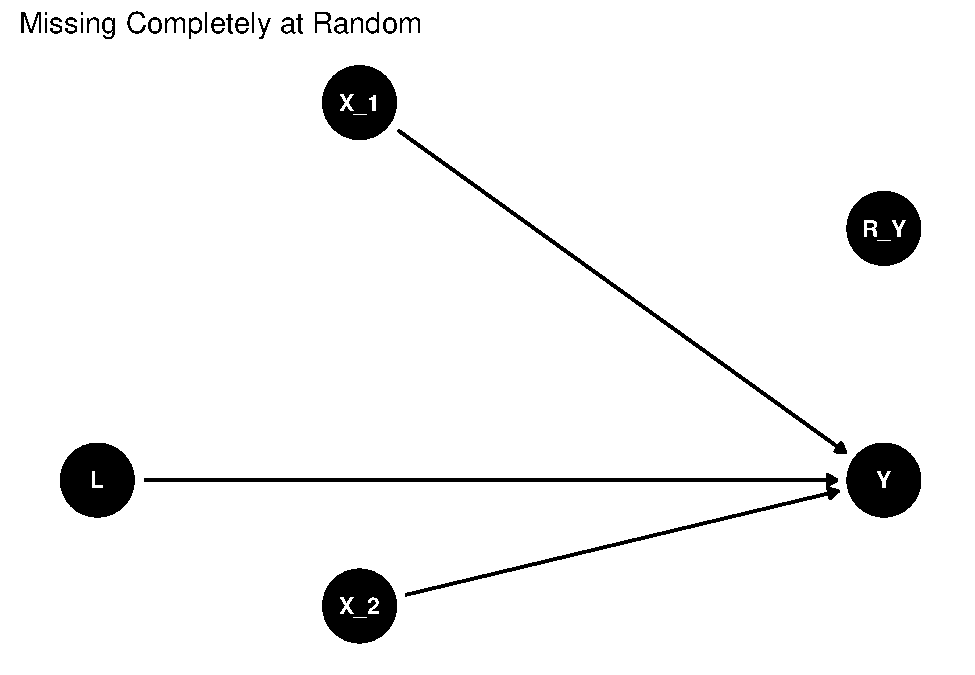
\includegraphics[keepaspectratio]{Final_Report_files/figure-latex/unnamed-chunk-1-1.pdf}}

\begin{Shaded}
\begin{Highlighting}[]
\NormalTok{acu\_miss\_perc\_group}
\end{Highlighting}
\end{Shaded}

\pandocbounded{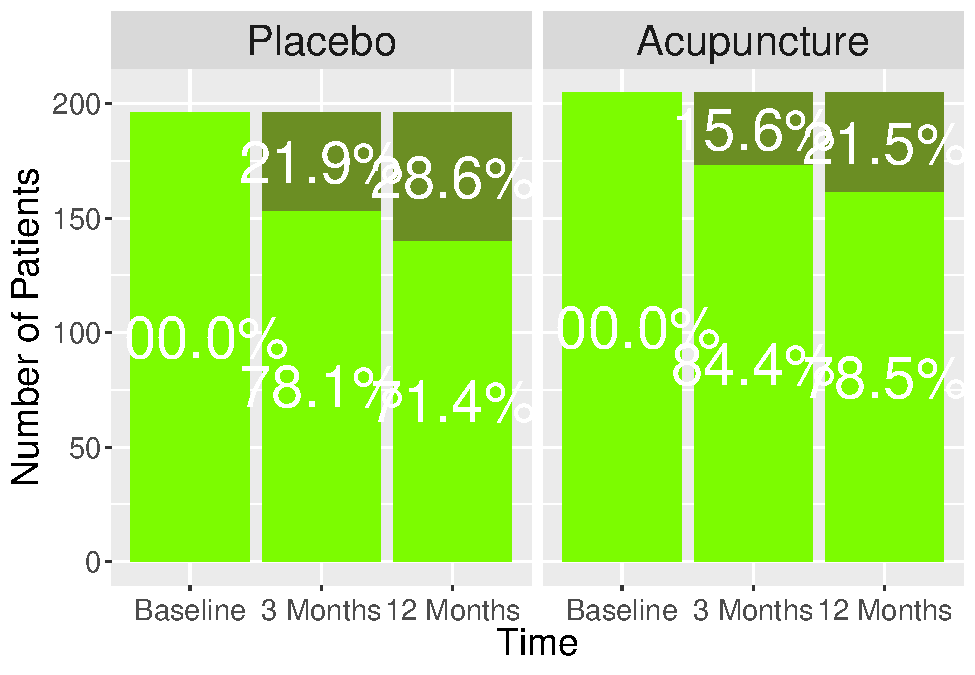
\includegraphics[keepaspectratio]{Final_Report_files/figure-latex/unnamed-chunk-1-2.pdf}}

\begin{Shaded}
\begin{Highlighting}[]
\NormalTok{acu\_miss\_pattern\_plot}
\end{Highlighting}
\end{Shaded}

\pandocbounded{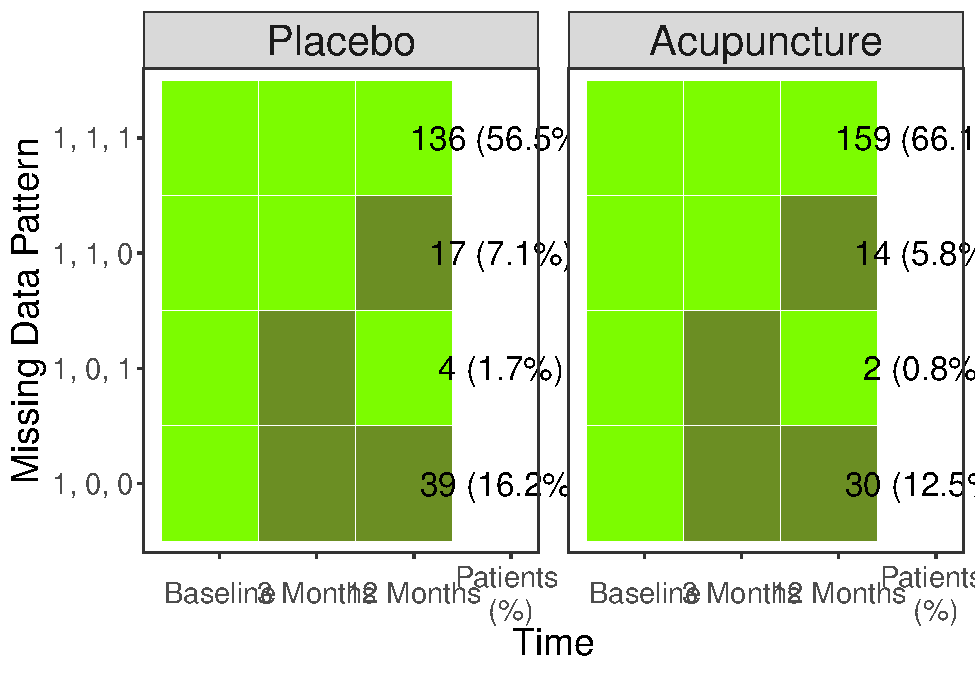
\includegraphics[keepaspectratio]{Final_Report_files/figure-latex/unnamed-chunk-1-3.pdf}}
-estimands

\subsection{The Effects of Vitamin D and Marine Omega-3 Fatty Acid
Supplementation on Chronic Knee Pain in Older US Adults: Results From a
Randomized Trial (MacFarlane et
al.~2020)}\label{the-effects-of-vitamin-d-and-marine-omega-3-fatty-acid-supplementation-on-chronic-knee-pain-in-older-us-adults-results-from-a-randomized-trial-macfarlane-et-al.-2020}

\textbf{Study Design}

\textbf{Characteristics}

table summary

\textbf{Missing Data}

\begin{Shaded}
\begin{Highlighting}[]
\NormalTok{vital\_miss\_perc\_plot}
\end{Highlighting}
\end{Shaded}

\pandocbounded{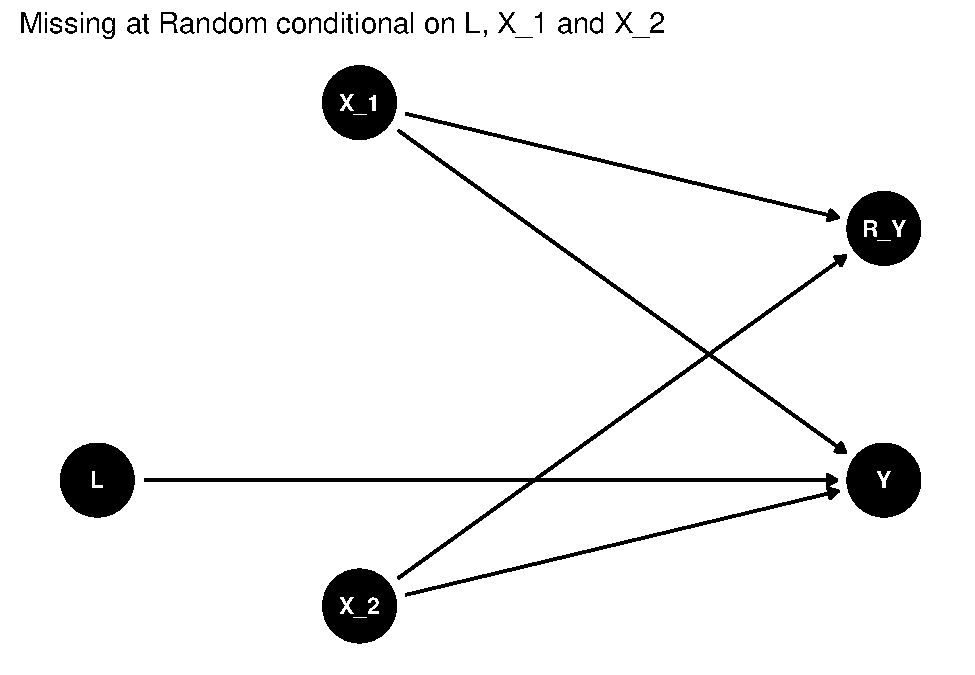
\includegraphics[keepaspectratio]{Final_Report_files/figure-latex/unnamed-chunk-2-1.pdf}}

\begin{Shaded}
\begin{Highlighting}[]
\NormalTok{vital\_miss\_perc\_plot\_fish}
\end{Highlighting}
\end{Shaded}

\pandocbounded{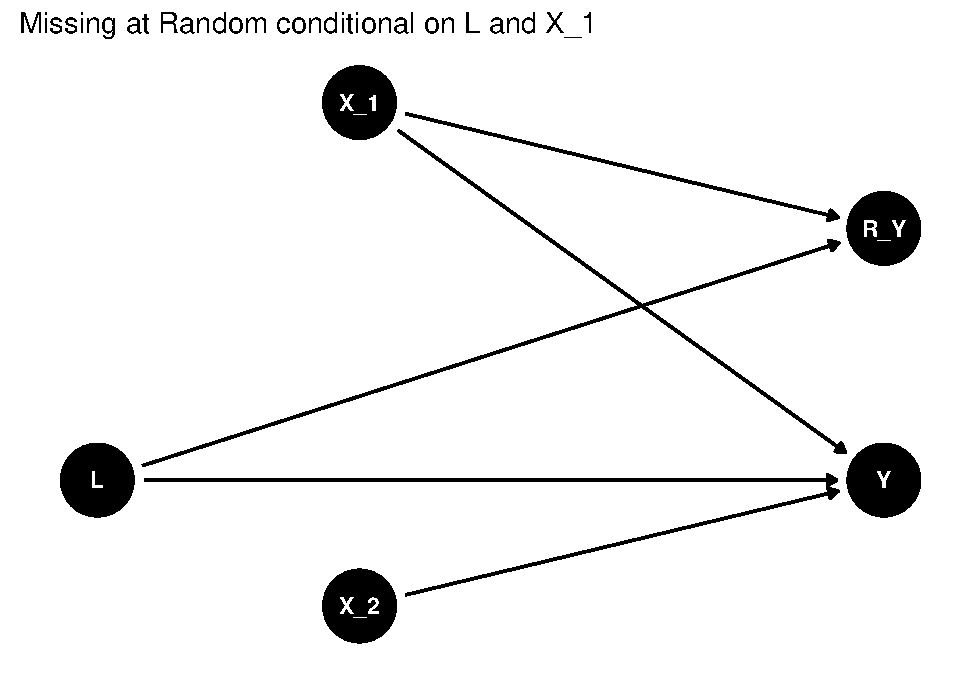
\includegraphics[keepaspectratio]{Final_Report_files/figure-latex/unnamed-chunk-2-2.pdf}}

\begin{Shaded}
\begin{Highlighting}[]
\NormalTok{vital\_miss\_pattern\_fish}
\end{Highlighting}
\end{Shaded}

\pandocbounded{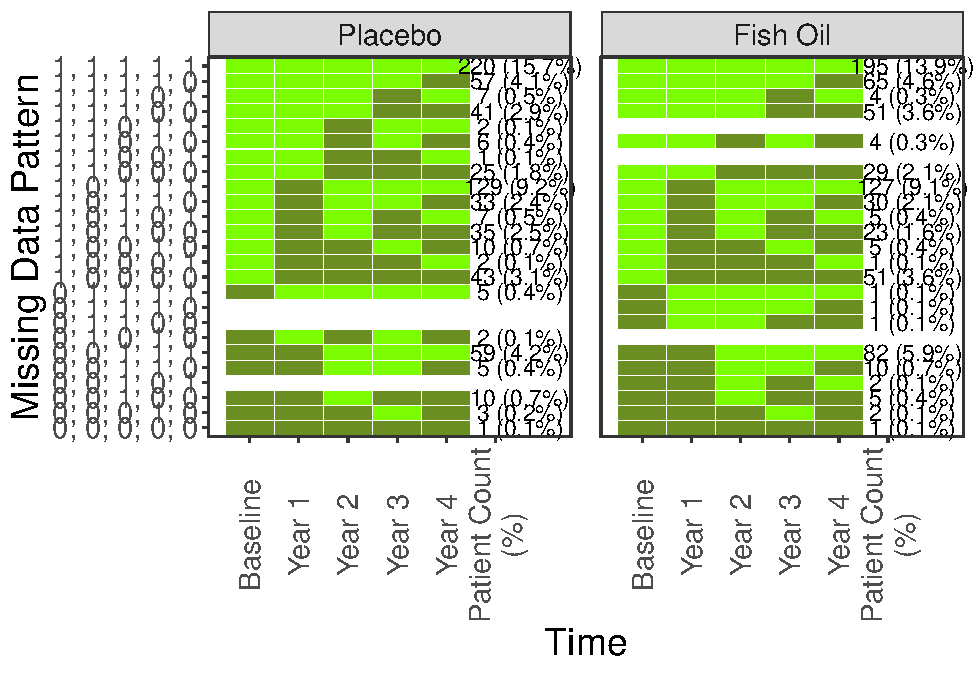
\includegraphics[keepaspectratio]{Final_Report_files/figure-latex/unnamed-chunk-2-3.pdf}}
- estimand

\subsection{Methods}\label{methods-1}

\subsection{Complete Case Analysis}\label{complete-case-analysis}

\begin{itemize}
\tightlist
\item
  method
\item
  mcar
\end{itemize}

\subsection{Single Imputation}\label{single-imputation}

mean locf mcar

\subsection{Maximum Likelihood}\label{maximum-likelihood}

\begin{itemize}
\tightlist
\item
  linear mixed effects model
\item
  conditions
\item
  only suitable with missing outcome
\item
  mar
\end{itemize}

\subsection{Multiple Imputation}\label{multiple-imputation}

\begin{itemize}
\tightlist
\item
  chained equations
\item
  mar
\end{itemize}

\subsection{Sensitivity Analysis}\label{sensitivity-analysis}

\subsection{Results}\label{results}

forest plots table of estimates sensitivity analysis

\section{Examples of citations, figures, tables,
references}\label{examples-of-citations-figures-tables-references}

\label{sec:others}

You can insert references. Here is some text (\textbf{kour2014real?};
\textbf{kour2014fast?}) and see (\textbf{hadash2018estimate?}).

The documentation for \verb+natbib+ may be found at

You can use custom blocks with LaTeX support from \textbf{rmarkdown} to
create environment.

\begin{center}
\url{http://mirrors.ctan.org/macros/latex/contrib/natbib/natnotes.pdf\%7D}

\end{center}

Of note is the command \verb+\citet+, which produces citations
appropriate for use in inline text.

You can insert LaTeX environment directly too.

\begin{verbatim}
   \citet{hasselmo} investigated\dots
\end{verbatim}

produces

\begin{quote}
  Hasselmo, et al.\ (1995) investigated\dots
\end{quote}

\begin{center}
  \url{https://www.ctan.org/pkg/booktabs}
\end{center}

\subsection{Figures}\label{figures}

You can insert figure using LaTeX directly.

See Figure \ref{fig:fig1}. Here is how you add footnotes. {[}\^{}Sample
of the first footnote.{]}

\begin{figure}
  \centering
  \fbox{\rule[-.5cm]{4cm}{4cm} \rule[-.5cm]{4cm}{0cm}}
  \caption{Sample figure caption.}
  \label{fig:fig1}
\end{figure}

But you can also do that using R.

\begin{Shaded}
\begin{Highlighting}[]
\FunctionTok{plot}\NormalTok{(mtcars}\SpecialCharTok{$}\NormalTok{mpg)}
\end{Highlighting}
\end{Shaded}

\begin{figure}
\centering
\pandocbounded{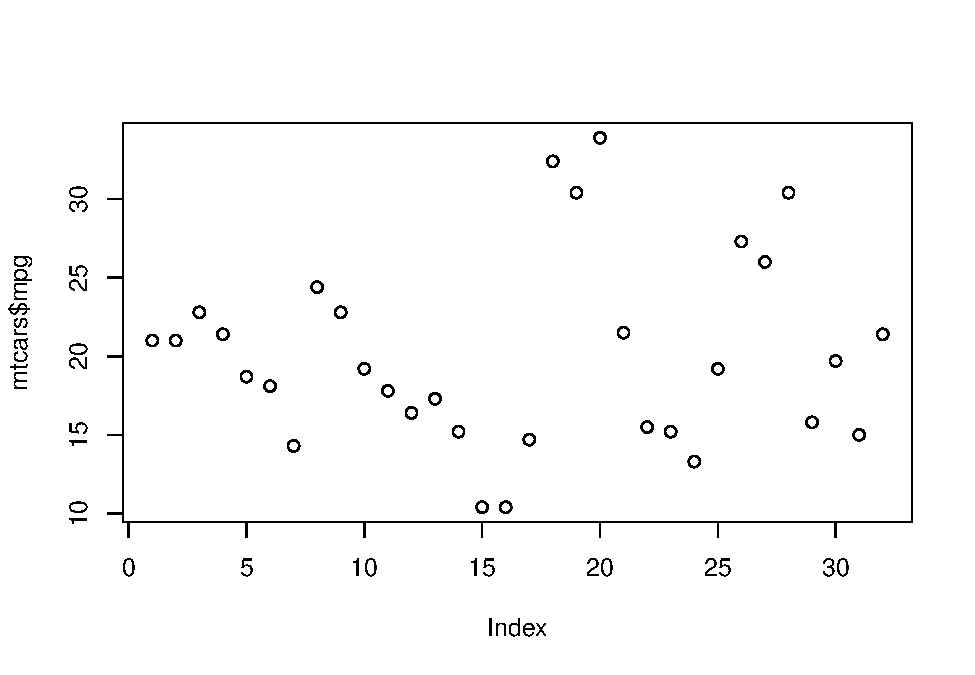
\includegraphics[keepaspectratio]{Final_Report_files/figure-latex/fig2-1.pdf}}
\caption{Another sample figure}
\end{figure}

You can use \textbf{bookdown} to allow references for Tables and
Figures.

\subsection{Tables}\label{tables}

Below we can see how to use tables.

See awesome Table\textasciitilde{}\ref{tab:table} which is written
directly in LaTeX in source Rmd file.

\begin{table}
 \caption{Sample table title}
  \centering
  \begin{tabular}{lll}
    \toprule
    \multicolumn{2}{c}{Part}                   \\
    \cmidrule(r){1-2}
    Name     & Description     & Size ($\mu$m) \\
    \midrule
    Dendrite & Input terminal  & $\sim$100     \\
    Axon     & Output terminal & $\sim$10      \\
    Soma     & Cell body       & up to $10^6$  \\
    \bottomrule
  \end{tabular}
  \label{tab:table}
\end{table}

You can also use R code for that.

\begin{Shaded}
\begin{Highlighting}[]
\NormalTok{knitr}\SpecialCharTok{::}\FunctionTok{kable}\NormalTok{(}\FunctionTok{head}\NormalTok{(mtcars), }\AttributeTok{caption =} \StringTok{"Head of mtcars table"}\NormalTok{)}
\end{Highlighting}
\end{Shaded}

\begin{longtable}[]{@{}
  >{\raggedright\arraybackslash}p{(\linewidth - 22\tabcolsep) * \real{0.2609}}
  >{\raggedleft\arraybackslash}p{(\linewidth - 22\tabcolsep) * \real{0.0725}}
  >{\raggedleft\arraybackslash}p{(\linewidth - 22\tabcolsep) * \real{0.0580}}
  >{\raggedleft\arraybackslash}p{(\linewidth - 22\tabcolsep) * \real{0.0725}}
  >{\raggedleft\arraybackslash}p{(\linewidth - 22\tabcolsep) * \real{0.0580}}
  >{\raggedleft\arraybackslash}p{(\linewidth - 22\tabcolsep) * \real{0.0725}}
  >{\raggedleft\arraybackslash}p{(\linewidth - 22\tabcolsep) * \real{0.0870}}
  >{\raggedleft\arraybackslash}p{(\linewidth - 22\tabcolsep) * \real{0.0870}}
  >{\raggedleft\arraybackslash}p{(\linewidth - 22\tabcolsep) * \real{0.0435}}
  >{\raggedleft\arraybackslash}p{(\linewidth - 22\tabcolsep) * \real{0.0435}}
  >{\raggedleft\arraybackslash}p{(\linewidth - 22\tabcolsep) * \real{0.0725}}
  >{\raggedleft\arraybackslash}p{(\linewidth - 22\tabcolsep) * \real{0.0725}}@{}}
\caption{Head of mtcars table}\tabularnewline
\toprule\noalign{}
\begin{minipage}[b]{\linewidth}\raggedright
\end{minipage} & \begin{minipage}[b]{\linewidth}\raggedleft
mpg
\end{minipage} & \begin{minipage}[b]{\linewidth}\raggedleft
cyl
\end{minipage} & \begin{minipage}[b]{\linewidth}\raggedleft
disp
\end{minipage} & \begin{minipage}[b]{\linewidth}\raggedleft
hp
\end{minipage} & \begin{minipage}[b]{\linewidth}\raggedleft
drat
\end{minipage} & \begin{minipage}[b]{\linewidth}\raggedleft
wt
\end{minipage} & \begin{minipage}[b]{\linewidth}\raggedleft
qsec
\end{minipage} & \begin{minipage}[b]{\linewidth}\raggedleft
vs
\end{minipage} & \begin{minipage}[b]{\linewidth}\raggedleft
am
\end{minipage} & \begin{minipage}[b]{\linewidth}\raggedleft
gear
\end{minipage} & \begin{minipage}[b]{\linewidth}\raggedleft
carb
\end{minipage} \\
\midrule\noalign{}
\endfirsthead
\toprule\noalign{}
\begin{minipage}[b]{\linewidth}\raggedright
\end{minipage} & \begin{minipage}[b]{\linewidth}\raggedleft
mpg
\end{minipage} & \begin{minipage}[b]{\linewidth}\raggedleft
cyl
\end{minipage} & \begin{minipage}[b]{\linewidth}\raggedleft
disp
\end{minipage} & \begin{minipage}[b]{\linewidth}\raggedleft
hp
\end{minipage} & \begin{minipage}[b]{\linewidth}\raggedleft
drat
\end{minipage} & \begin{minipage}[b]{\linewidth}\raggedleft
wt
\end{minipage} & \begin{minipage}[b]{\linewidth}\raggedleft
qsec
\end{minipage} & \begin{minipage}[b]{\linewidth}\raggedleft
vs
\end{minipage} & \begin{minipage}[b]{\linewidth}\raggedleft
am
\end{minipage} & \begin{minipage}[b]{\linewidth}\raggedleft
gear
\end{minipage} & \begin{minipage}[b]{\linewidth}\raggedleft
carb
\end{minipage} \\
\midrule\noalign{}
\endhead
\bottomrule\noalign{}
\endlastfoot
Mazda RX4 & 21.0 & 6 & 160 & 110 & 3.90 & 2.620 & 16.46 & 0 & 1 & 4 &
4 \\
Mazda RX4 Wag & 21.0 & 6 & 160 & 110 & 3.90 & 2.875 & 17.02 & 0 & 1 & 4
& 4 \\
Datsun 710 & 22.8 & 4 & 108 & 93 & 3.85 & 2.320 & 18.61 & 1 & 1 & 4 &
1 \\
Hornet 4 Drive & 21.4 & 6 & 258 & 110 & 3.08 & 3.215 & 19.44 & 1 & 0 & 3
& 1 \\
Hornet Sportabout & 18.7 & 8 & 360 & 175 & 3.15 & 3.440 & 17.02 & 0 & 0
& 3 & 2 \\
Valiant & 18.1 & 6 & 225 & 105 & 2.76 & 3.460 & 20.22 & 1 & 0 & 3 & 1 \\
\end{longtable}

\subsection{Lists}\label{lists}

\begin{itemize}
\tightlist
\item
  Item 1
\item
  Item 2
\item
  Item 3
\end{itemize}

\bibliographystyle{unsrt}
\bibliography{references.bib}


\end{document}
